



\documentclass[12pt]{article}
% \usepackage[utf8]{inputenc}
% \usepackage{times} % This package sets the Times New Roman font

\usepackage{palatino} % This package sets the Times New Roman font

% \usepackage{newcent} % This package sets the Times New Roman font
\usepackage[T1]{fontenc}
\usepackage[a4paper, margin=1in]{geometry}

\usepackage{titlesec}

% 定义章节标题格式,包括字体大小、粗体
\titleformat{\section}
  {\normalfont\Large\bfseries}{\thesection}{1em}{}


% \usepackage{newtxtext}
\usepackage{amsmath,amssymb,amsthm}
\usepackage{newtxmath} % must come after amsXXX

\usepackage{float}%防止图片乱跑---真 防止图片乱跑,还得用[H]



\usepackage{graphicx}
%\usepackage{subfigure}
\usepackage{subcaption}


\usepackage{tikz}% to edit on imagines
\usetikzlibrary{spy}% to zoom the pictures
\usetikzlibrary{arrows.meta, positioning, calc} %to drawing
\usetikzlibrary{patterns} % to drawing

\usepackage{xcolor}
\usepackage{fancyhdr}

\usepackage{listings}
%\usepackage{ctex}

\usepackage{booktabs}


%%%%%%%%%%%% for sudocode %%%%%%%
\usepackage{algorithm}
\usepackage{algpseudocode}
%%%%%%%%%%%%%%%%%%%%%%%%%%%%%%%%%

%%%%%%%%%%%%%%%% Set Up code paste style (VS datk+ style)%%%%%%%%%%%%%%%%%
% Define custom colors
\definecolor{codepurple}{rgb}{0.58,0,0.82}
\definecolor{codegray}{rgb}{0.5,0.5,0.5}
\definecolor{backcolour}{rgb}{0.95,0.95,0.92}

% Code listing style
\lstdefinestyle{mystyle}{
    language=Matlab,
    % backgroundcolor=\color{wight},
    frame=single,
    numbers=left,
    numbersep=10pt,
    basicstyle=\ttfamily,
    breaklines=true,
    showspaces=false,
    showstringspaces=false,
    showtabs=false
}

\lstset{style=mystyle}
%%%%%%%%%%%%%%%%%%%%%%%%%%%%%%%%%



% Examples:

% % Picture:
% \begin{figure}[H]
%     \centering
%     \includegraphics[width=1\textwidth]{figuresGeneral/Solver_Structure.jpg}
%     \label{IGs.jpg}
%     \caption{Solver Structure }
% \end{figure}

% % Algorithm:

% \begin{algorithm}[H]
%     \small
% \caption{xxx Method}
% \begin{algorithmic}[1]
% \For{ timestep = $n = 0$ to $N-1$} \Comment{Loop over time steps}
%     \State // Step from $n$ to $n+\frac{1}{2}$
%     \For{each each $j$ lines}  \Comment{Loop over each line}
%         \State a=b=c=($i_{max}$-1)x1 space, $a[i] = c[i] = a$, $b[i]  = b$
%         \State $U_{half}[i,j]$ = TDMA(a,b,c,d)
%     \EndFor
%     \State $U_{new}$ = BC($U_{new}$), $U = U_{new}$ 
% \EndFor

% \end{algorithmic}
% \end{algorithm}






%%%%%%%%%%%%%%%%%%%%%%%%%%%%%%%%%%%%%%%%%%%%%%%%%%%%%%%%%%%%%%%
%%%%%%%%%%%%%%%%%%%%%%%%%%%%%%%%%%%%%%%%%%%%%%%%%%%%%%%%%%%%%%%

\begin{document}

\title{\begin{Huge}Fluid Dynamics II\end{Huge}\\Haobo Zhao\\Mini Project-4}
\maketitle

\tableofcontents


\section{Question Review}

Using the Prandtl lifting line theory, calculate the aerodynamic coefficients of a wing for which aerodynamic data are available. The wing's geometry to be studied is illustrated in the figure below. The wing, which is unswept at the quarter chord, is composed of NACA 65-210 airfoil sections. The zero-lift angle of attack $(\alpha_{L=0})$ is approximately $-1.2$ across the span. Since the wing is untwisted, the geometric angle of attack is the same at all spanwise positions. The aspect ratio (AR) is $9.00$. The taper ratio $\lambda$ (i.e., $C_t/C_r$) is $0.40$. The wing planform is trapezoidal, as seen in the figure below.

Next, model this problem in Fluent (inviscid flow) and obtain the aerodynamic coefficients of the wing. Compare the results from the two methods (analytical, Fluent).

% Picture:
\begin{figure}[H]
    \centering
    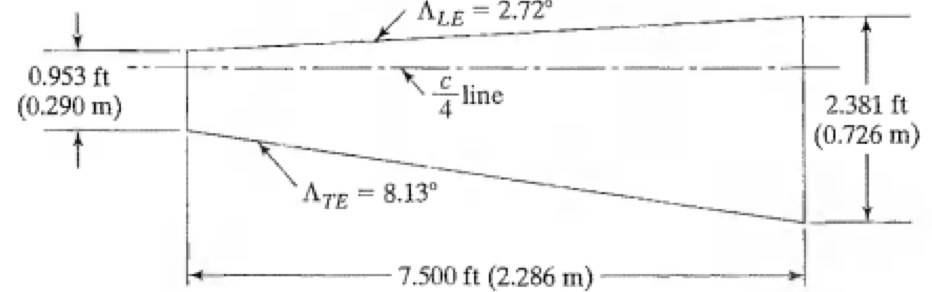
\includegraphics[width=0.8\textwidth]{Homeworks/fluids-MinProject4/Latex/figure/Win.jpg}
    \label{IGs.jpg}
\end{figure}






\section{Result Based on Prandtl Lifting Line Theory}

\subsection{Prandtl Lifting Line Theory}
Based on Prnadtl lifting theory, the formula we could get as follows:
$$
\alpha(\theta_0) = \frac{2b}{\pi C(\theta_0)} \sum_{n=1}^{N} A_n \sin(n \theta_0) + \alpha_{L=0}(\theta_0) + \sum_{n=1}^{N} n A_n \frac{\sin n \theta}{\sin \theta_0}
$$

To get $An$, we need to build a matrix equation based on different $\theta_0$. As $\theta_0$ is based on $y$, which is showing below:
$$
y = \frac{b}{2} \cos \theta
$$

We could choose \# N different $y$ or $\theta_0$ among the wing, could get \# N of An, which means we are building an $N \times N$ matrix:
$$
\sum_{i=1}^{n} \left[ \frac{2b}{\pi C(\theta_0)} \sin(n \theta_0) + n \frac{\sin(n \theta_0)}{\sin(\theta_0)} \right] A_n = \alpha(\theta_0) - \alpha_{L=0}(\theta_0)
$$

Where, $An$ is variable, and $ \frac{2b}{\pi C(\theta_0)} \sin(n \theta_0) + n \frac{\sin(n \theta_0)}{\sin(\theta_0)}$ is the coefficient for each $An$. As the wing is untwisted, $\alpha_{L=0}(\theta_0)$ is same among different $y$.\\

Then, we could use \# N $y$ to find \# N $\theta_0$, and then find \# N $An$.\\



After we find $An$, we could calculate $C_l$ and $C_{Di}$ based on the following formula:
$$
C_L = A_1 \pi \frac{b^2}{s} = A_1 \pi AR
$$

and 

$$
C_{D_i} = \pi AR \left( A_1^2 +  \sum_{n=1}^{N} n A_n^2 \right)
$$

\subsection{Known variables}

\begin{table}[ht]
\centering
\begin{tabular}{cccccc}
\toprule
\( b \) & \( c_r \) & \( c_t \) & \( c \) & \( AR \) & \( \alpha_l \) \\
\midrule
\( 2.286 \times 2 \) & \( 0.290 \) & \( 0.726 \) & \( \frac{0.290 + 0.726}{2} \) & \( 9 \) & \( -1.2 \times \frac{\pi}{180} \) \\
\bottomrule
\end{tabular}
\caption{Variable Assignments}
\label{tab:variables}
\end{table}



\subsection{Code and algorithms}


\begin{lstlisting}[caption={A function for SD},label={lst:script1}]
angle = 6

b = 2.286*2;
c_r = 0.290;
c_t = 0.726;
c = (c_r +c_t)/2;
AR = 9;
a_l = -1.2*pi/180;

y_0  = 0;
y_max = b/2;
N = 99;
theta = linspace(0,pi,N);
theta = theta(2:N-1);
y = b/2 .* cos(theta);
c_y = c_r + (c_t - c_r)/(b/2) * (b/2-abs(y));
k1 = 2*b/pi./c_y;


matrix = zeros(N-2, N-2);
for i = 1:N-2
    for n = 1:N-2
        matrix(i,n) = k1(i) * sin(n.*theta(i)) + n*sin(n.*theta(i))/sin(theta(i));
    end
end

a= angle*pi/180;
rhs = ones(N-2)*(a-a_l);
An = matrix\rhs;
cl = An(1)*pi * AR

Summ = 0;
for n= 1:N-2
   Summ = Summ + n*(An(n))^2;
end

cdi = pi * AR * Summ
\end{lstlisting}









\subsection{Result of different angle of attack}


% Picture:
\begin{figure}[H]
    \centering
    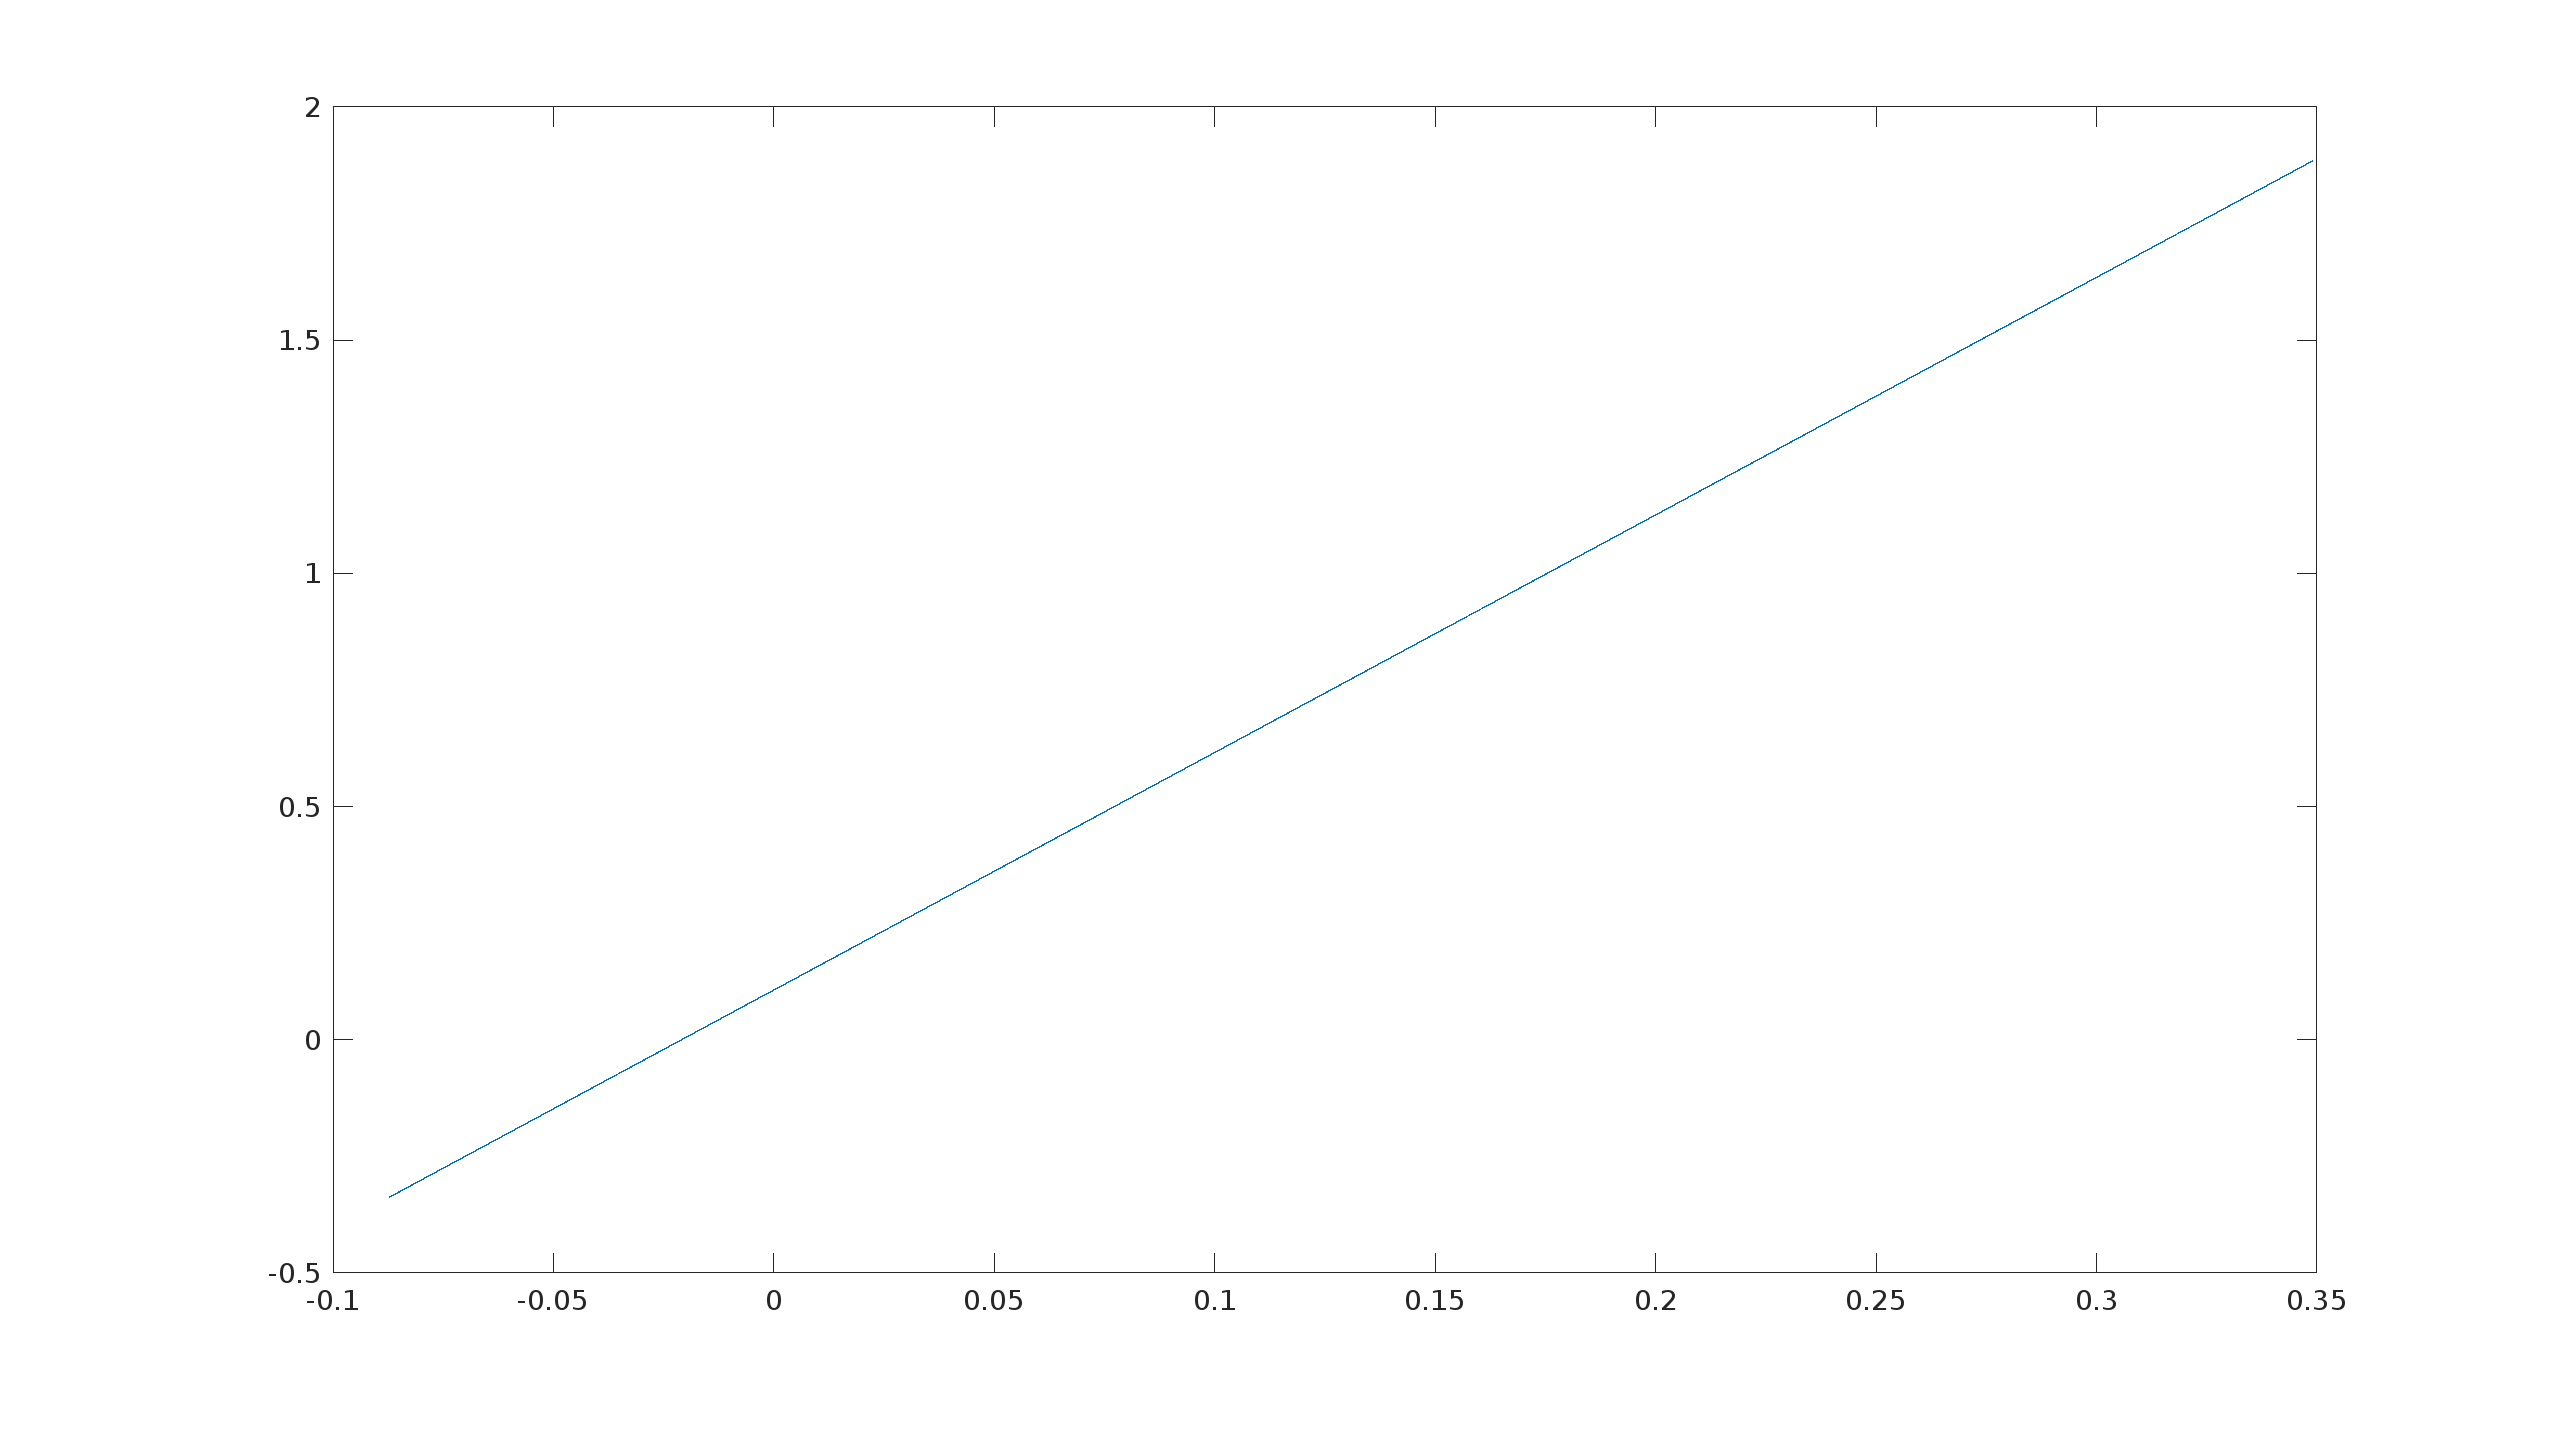
\includegraphics[width=1\textwidth]{Homeworks/fluids-MinProject4/Latex/figure/Cl.png}
    \label{IGs.jpg}
    \caption{$C_L$ for different angle of attack}
\end{figure}

% Picture:
\begin{figure}[H]
    \centering
    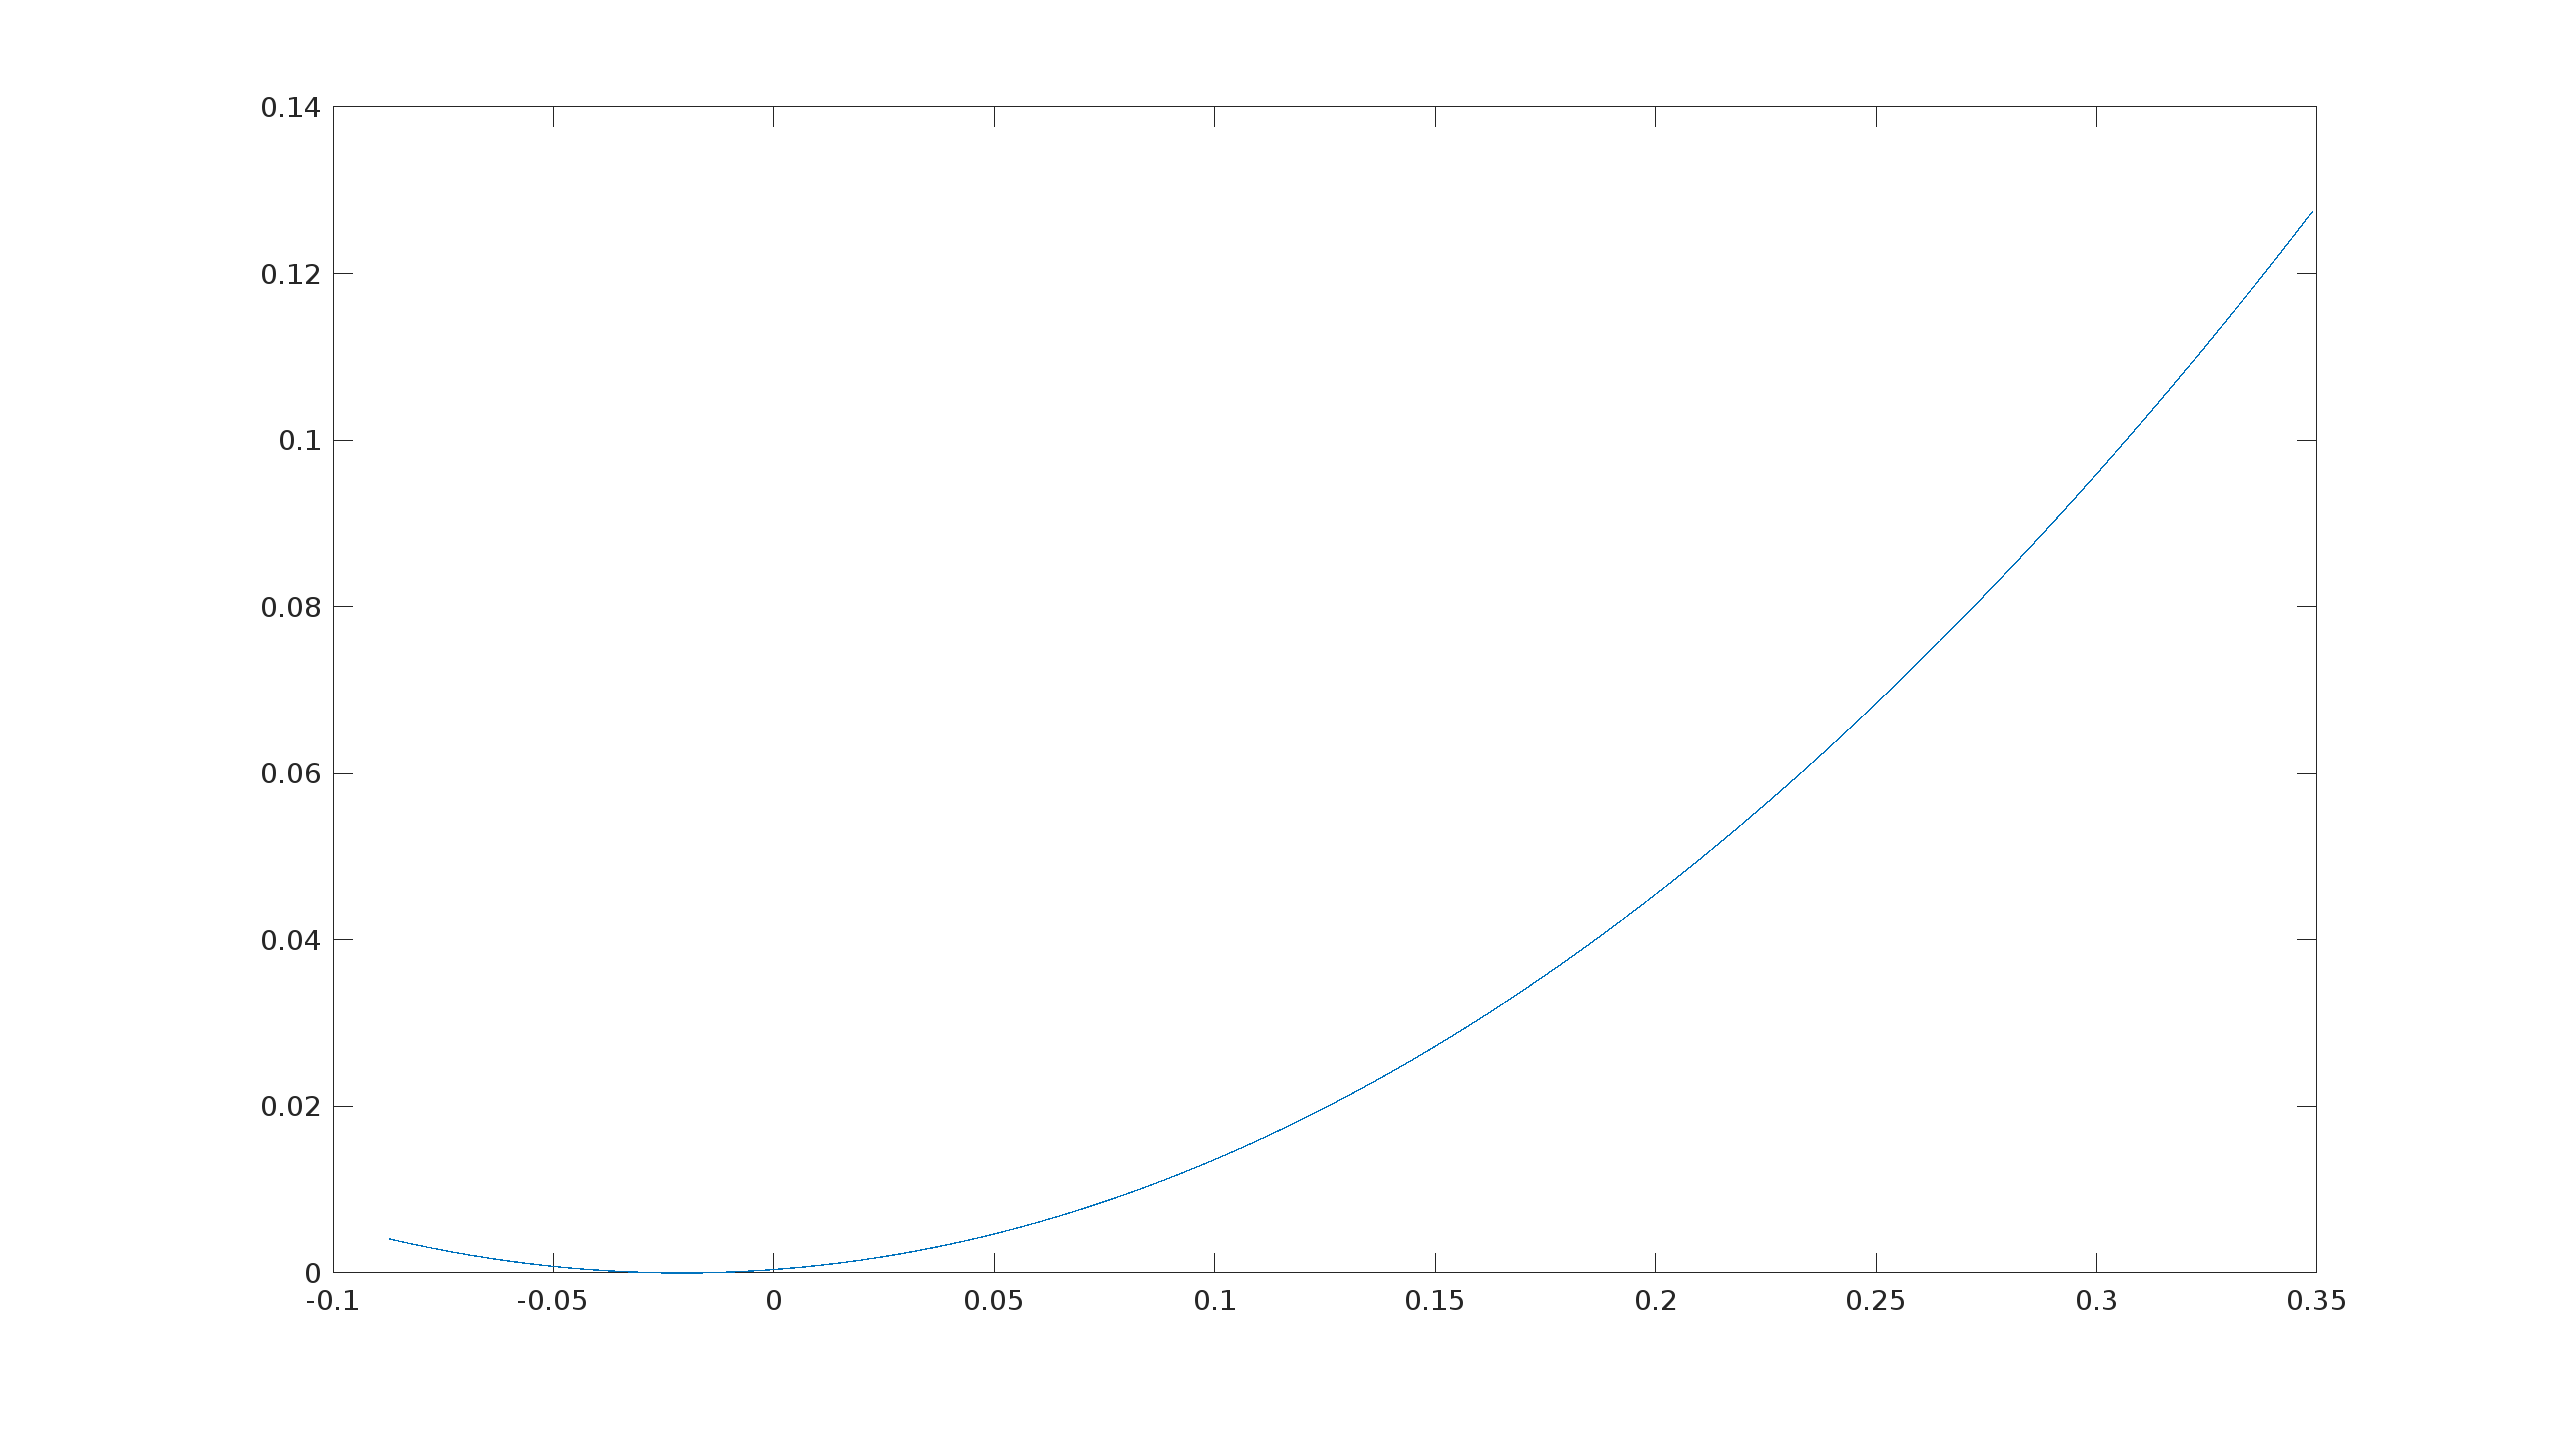
\includegraphics[width=1\textwidth]{Homeworks/fluids-MinProject4/Latex/figure/Cdi.png}
    \label{IGs.jpg}
    \caption{$C_{Di}$ for different angle of attack}
\end{figure}


\section{ANSYS Modeling for 3D-Wing}


\subsection{3D Modeling and Boundary setting}

By getting NACA-65-210 airfoil from website, we could create the 3D-model based on the diagram showned in the question.\\

We could get 3D model as follows:
% Picture:
\begin{figure}[H]
    \centering
    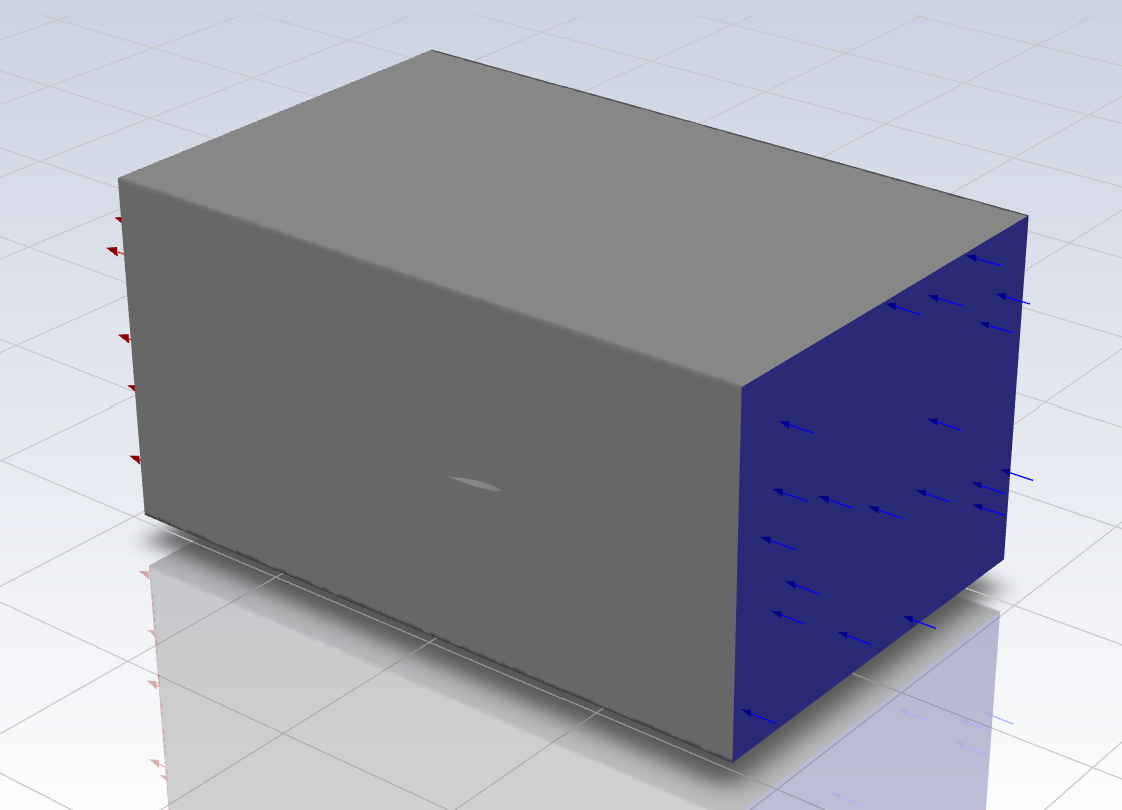
\includegraphics[width=0.6\textwidth]{Homeworks/fluids-MinProject4/Latex/figure/3D-Model.png}
    \label{IGs.jpg}
    \caption{3D model}
\end{figure}






After we got the 3D geometry of the calculation domain, we need to set the boundaries:

% Picture:
\begin{figure}[H]
    \centering
    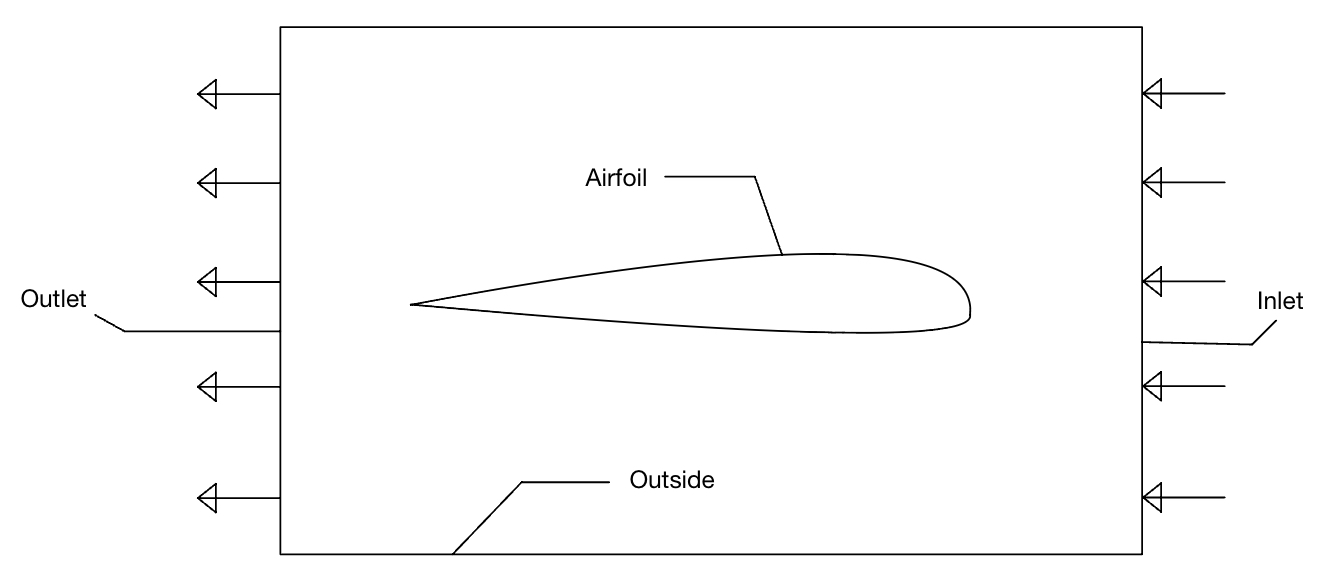
\includegraphics[width=1\textwidth]{Homeworks/fluids-MinProject4/Latex/figure/diagram-2D.jpg}
    \label{IGs.jpg}
    \caption{2D boundary define}
\end{figure}

This is our model in 2D-view, from which we can find there is 4 kind of boundaries: Inlet, outlet, airfoil, and outside:
\begin{itemize}
    \item Inlet: air velocity inlet, $v_in = 1m/s$
    \item Outlet: air outlet, $p=0$
    \item Airfoil: slip airfoil, as viscosity is 0
    \item Outside: outer boundary, symmetric
\end{itemize}


% Picture:
\begin{figure}[H]
    \centering
    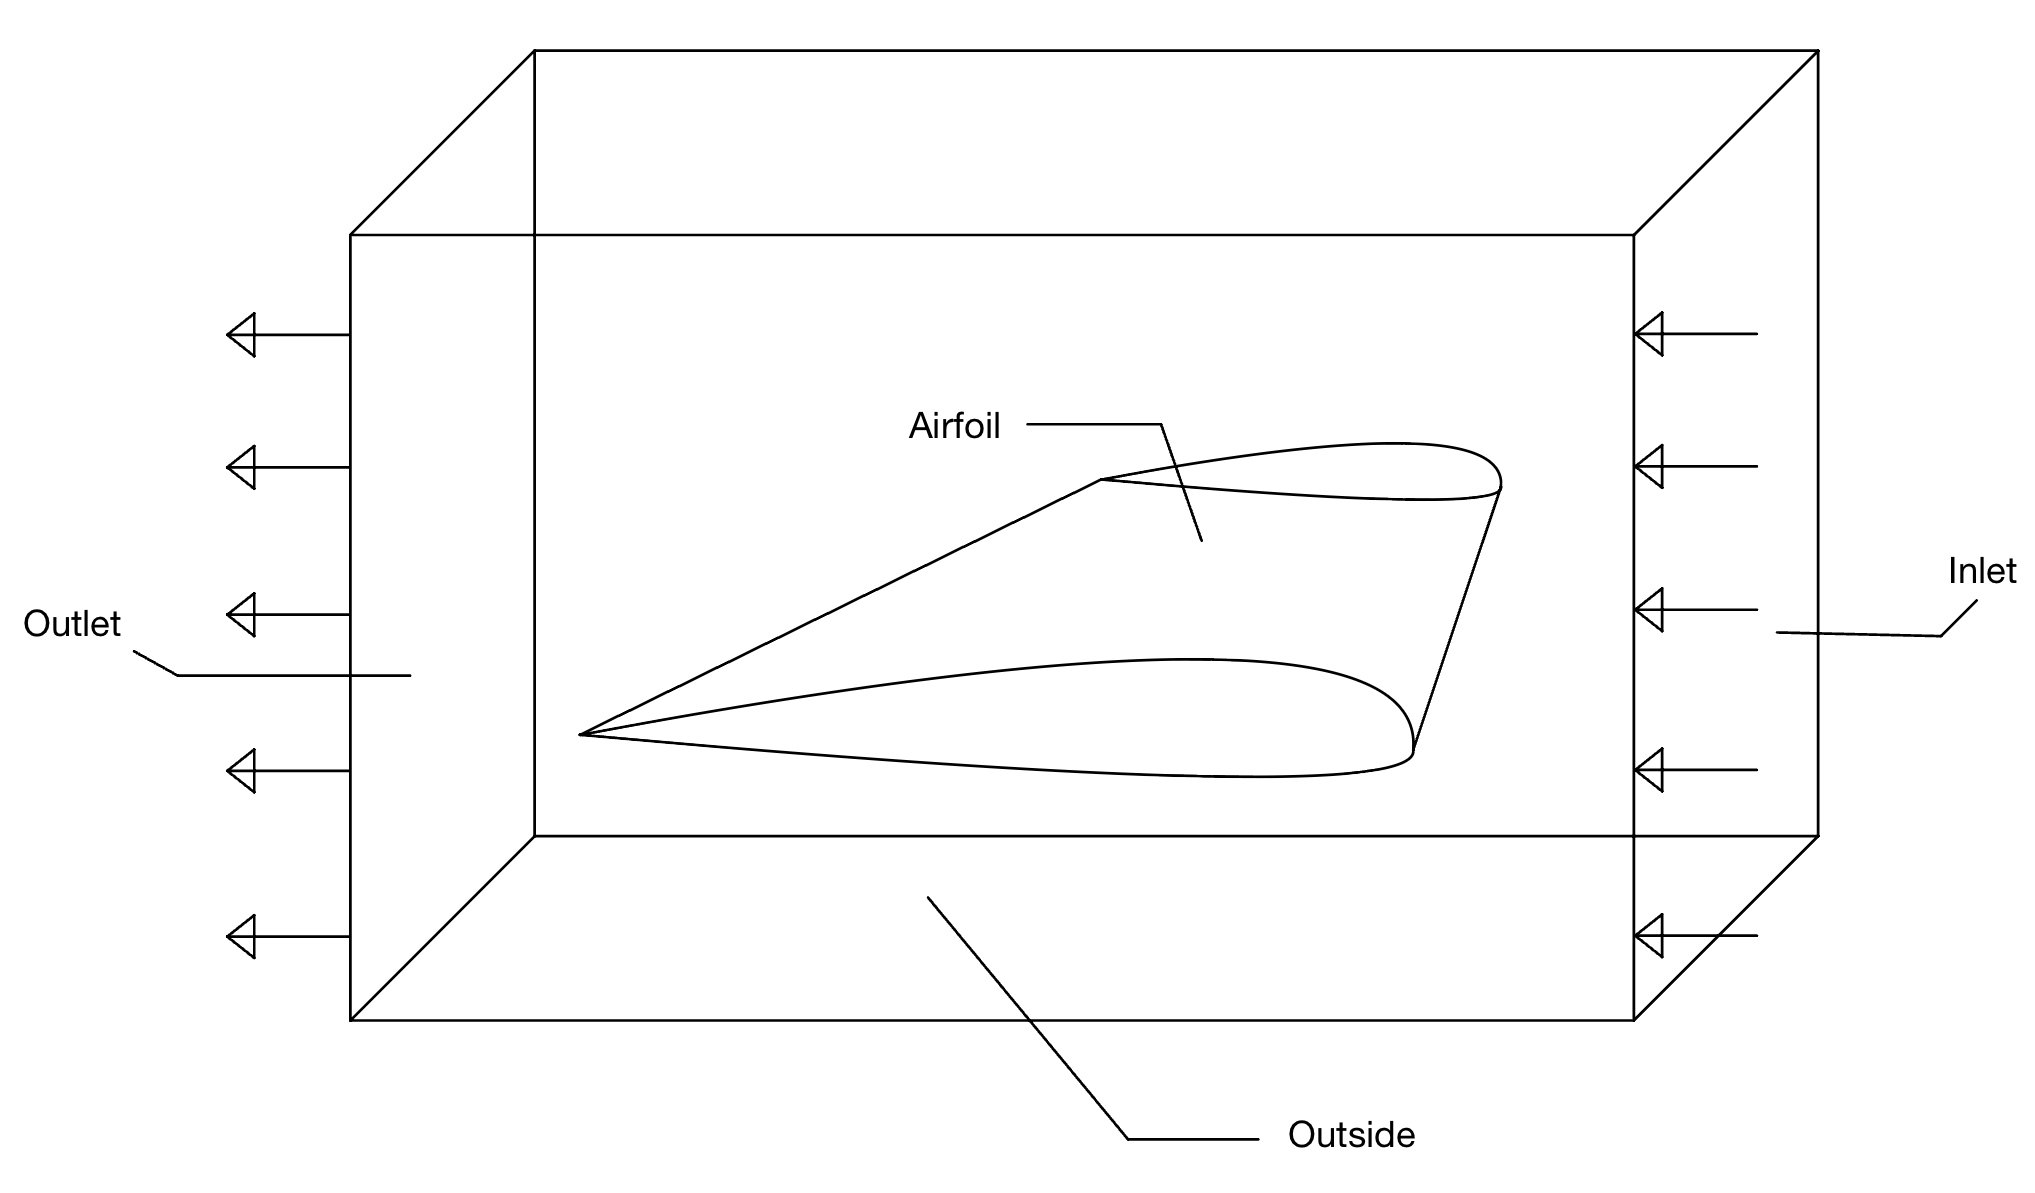
\includegraphics[width=0.6\textwidth]{Homeworks/fluids-MinProject4/Latex/figure/diagram-3D.jpg}
    \label{IGs.jpg}
    \caption{Geometry and boundary Setting in 3D view}
\end{figure}













\subsection{Result}

























\end{document}